\documentclass[1p]{elsarticle_modified}
%\bibliographystyle{elsarticle-num}

%\usepackage[colorlinks]{hyperref}
%\usepackage{abbrmath_seonhwa} %\Abb, \Ascr, \Acal ,\Abf, \Afrak
\usepackage{amsfonts}
\usepackage{amssymb}
\usepackage{amsmath}
\usepackage{amsthm}
\usepackage{scalefnt}
\usepackage{amsbsy}
\usepackage{kotex}
\usepackage{caption}
\usepackage{subfig}
\usepackage{color}
\usepackage{graphicx}
\usepackage{xcolor} %% white, black, red, green, blue, cyan, magenta, yellow
\usepackage{float}
\usepackage{setspace}
\usepackage{hyperref}

\usepackage{tikz}
\usetikzlibrary{arrows}

\usepackage{multirow}
\usepackage{array} % fixed length table
\usepackage{hhline}

%%%%%%%%%%%%%%%%%%%%%
\makeatletter
\renewcommand*\env@matrix[1][\arraystretch]{%
	\edef\arraystretch{#1}%
	\hskip -\arraycolsep
	\let\@ifnextchar\new@ifnextchar
	\array{*\c@MaxMatrixCols c}}
\makeatother %https://tex.stackexchange.com/questions/14071/how-can-i-increase-the-line-spacing-in-a-matrix
%%%%%%%%%%%%%%%

\usepackage[normalem]{ulem}

\newcommand{\msout}[1]{\ifmmode\text{\sout{\ensuremath{#1}}}\else\sout{#1}\fi}
%SOURCE: \msout is \stkout macro in https://tex.stackexchange.com/questions/20609/strikeout-in-math-mode

\newcommand{\cancel}[1]{
	\ifmmode
	{\color{red}\msout{#1}}
	\else
	{\color{red}\sout{#1}}
	\fi
}

\newcommand{\add}[1]{
	{\color{blue}\uwave{#1}}
}

\newcommand{\replace}[2]{
	\ifmmode
	{\color{red}\msout{#1}}{\color{blue}\uwave{#2}}
	\else
	{\color{red}\sout{#1}}{\color{blue}\uwave{#2}}
	\fi
}

\newcommand{\Sol}{\mathcal{S}} %segment
\newcommand{\D}{D} %diagram
\newcommand{\A}{\mathcal{A}} %arc


%%%%%%%%%%%%%%%%%%%%%%%%%%%%%5 test

\def\sl{\operatorname{\textup{SL}}(2,\Cbb)}
\def\psl{\operatorname{\textup{PSL}}(2,\Cbb)}
\def\quan{\mkern 1mu \triangleright \mkern 1mu}

\theoremstyle{definition}
\newtheorem{thm}{Theorem}[section]
\newtheorem{prop}[thm]{Proposition}
\newtheorem{lem}[thm]{Lemma}
\newtheorem{ques}[thm]{Question}
\newtheorem{cor}[thm]{Corollary}
\newtheorem{defn}[thm]{Definition}
\newtheorem{exam}[thm]{Example}
\newtheorem{rmk}[thm]{Remark}
\newtheorem{alg}[thm]{Algorithm}

\newcommand{\I}{\sqrt{-1}}
\begin{document}

%\begin{frontmatter}
%
%\title{Boundary parabolic representations of knots up to 8 crossings}
%
%%% Group authors per affiliation:
%\author{Yunhi Cho} 
%\address{Department of Mathematics, University of Seoul, Seoul, Korea}
%\ead{yhcho@uos.ac.kr}
%
%
%\author{Seonhwa Kim} %\fnref{s_kim}}
%\address{Center for Geometry and Physics, Institute for Basic Science, Pohang, 37673, Korea}
%\ead{ryeona17@ibs.re.kr}
%
%\author{Hyuk Kim}
%\address{Department of Mathematical Sciences, Seoul National University, Seoul 08826, Korea}
%\ead{hyukkim@snu.ac.kr}
%
%\author{Seokbeom Yoon}
%\address{Department of Mathematical Sciences, Seoul National University, Seoul, 08826,  Korea}
%\ead{sbyoon15@snu.ac.kr}
%
%\begin{abstract}
%We find all boundary parabolic representation of knots up to 8 crossings.
%
%\end{abstract}
%\begin{keyword}
%    \MSC[2010] 57M25 
%\end{keyword}
%
%\end{frontmatter}

%\linenumbers
%\tableofcontents
%
\newcommand\colored[1]{\textcolor{white}{\rule[-0.35ex]{0.8em}{1.4ex}}\kern-0.8em\color{red} #1}%
%\newcommand\colored[1]{\textcolor{white}{ #1}\kern-2.17ex	\textcolor{white}{ #1}\kern-1.81ex	\textcolor{white}{ #1}\kern-2.15ex\color{red}#1	}

{\Large $\underline{11a_{224}~(K11a_{224})}$}

\setlength{\tabcolsep}{10pt}
\renewcommand{\arraystretch}{1.6}
\vspace{1cm}\begin{tabular}{m{100pt}>{\centering\arraybackslash}m{274pt}}
\multirow{5}{120pt}{
	\centering
	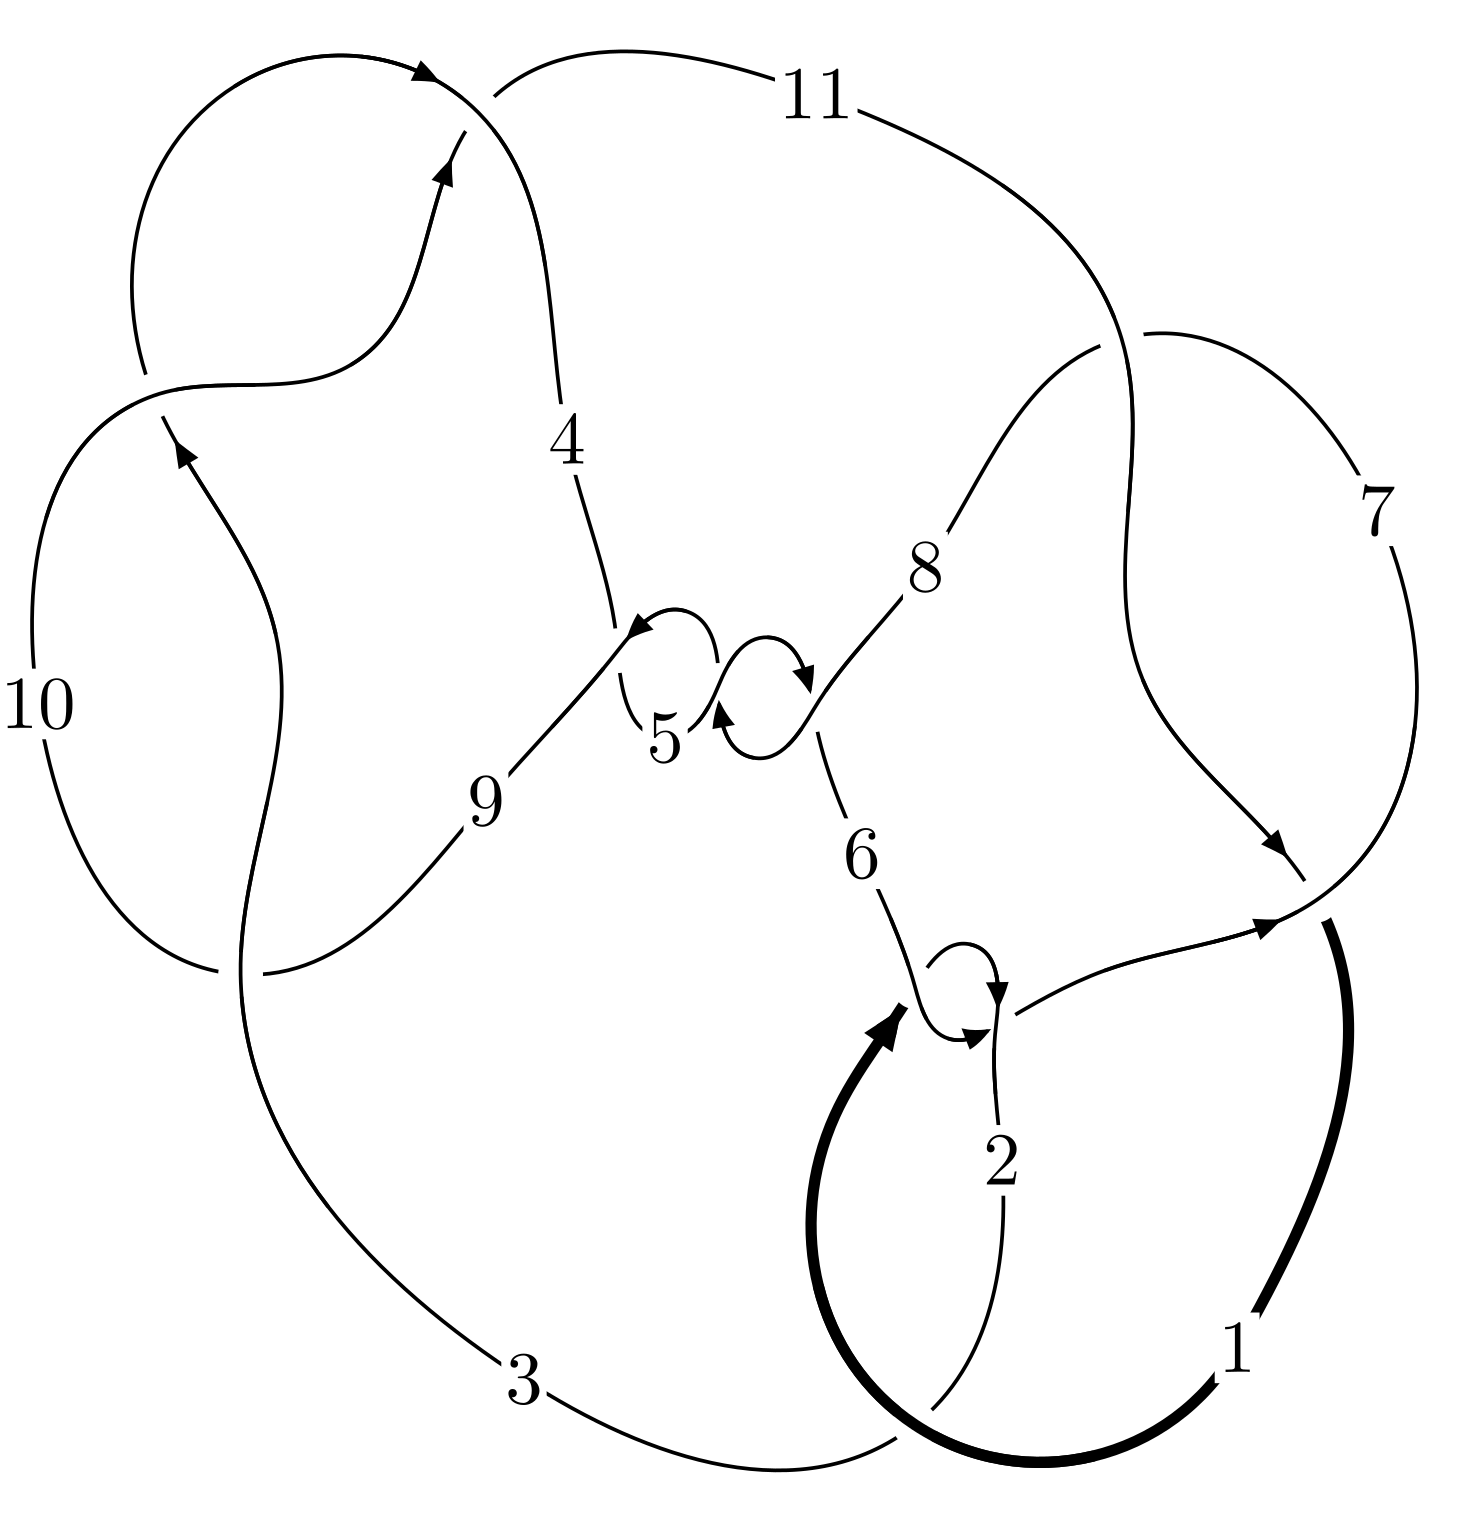
\includegraphics[width=112pt]{../../../GIT/diagram.site/Diagrams/png/473_11a_224.png}\\
\ \ \ A knot diagram\footnotemark}&
\allowdisplaybreaks
\textbf{Linearized knot diagam} \\
\cline{2-2}
 &
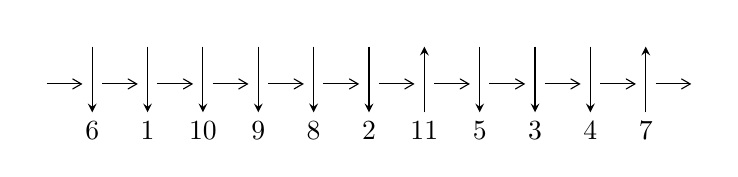
\begin{tikzpicture}[x=20pt, y=17pt]
	% nodes
	\node (C0) at (0, 0) {};
	\node (C1) at (1, 0) {};
	\node (C1U) at (1, +1) {};
	\node (C1D) at (1, -1) {6};

	\node (C2) at (2, 0) {};
	\node (C2U) at (2, +1) {};
	\node (C2D) at (2, -1) {1};

	\node (C3) at (3, 0) {};
	\node (C3U) at (3, +1) {};
	\node (C3D) at (3, -1) {10};

	\node (C4) at (4, 0) {};
	\node (C4U) at (4, +1) {};
	\node (C4D) at (4, -1) {9};

	\node (C5) at (5, 0) {};
	\node (C5U) at (5, +1) {};
	\node (C5D) at (5, -1) {8};

	\node (C6) at (6, 0) {};
	\node (C6U) at (6, +1) {};
	\node (C6D) at (6, -1) {2};

	\node (C7) at (7, 0) {};
	\node (C7U) at (7, +1) {};
	\node (C7D) at (7, -1) {11};

	\node (C8) at (8, 0) {};
	\node (C8U) at (8, +1) {};
	\node (C8D) at (8, -1) {5};

	\node (C9) at (9, 0) {};
	\node (C9U) at (9, +1) {};
	\node (C9D) at (9, -1) {3};

	\node (C10) at (10, 0) {};
	\node (C10U) at (10, +1) {};
	\node (C10D) at (10, -1) {4};

	\node (C11) at (11, 0) {};
	\node (C11U) at (11, +1) {};
	\node (C11D) at (11, -1) {7};
	\node (C12) at (12, 0) {};

	% arrows
	\draw[->,>={angle 60}]
	(C0) edge (C1) (C1) edge (C2) (C2) edge (C3) (C3) edge (C4) (C4) edge (C5) (C5) edge (C6) (C6) edge (C7) (C7) edge (C8) (C8) edge (C9) (C9) edge (C10) (C10) edge (C11) (C11) edge (C12) ;	\draw[->,>=stealth]
	(C1U) edge (C1D) (C2U) edge (C2D) (C3U) edge (C3D) (C4U) edge (C4D) (C5U) edge (C5D) (C6U) edge (C6D) (C7D) edge (C7U) (C8U) edge (C8D) (C9U) edge (C9D) (C10U) edge (C10D) (C11D) edge (C11U) ;
	\end{tikzpicture} \\
\hhline{~~} \\& 
\textbf{Solving Sequence} \\ \cline{2-2} 
 &
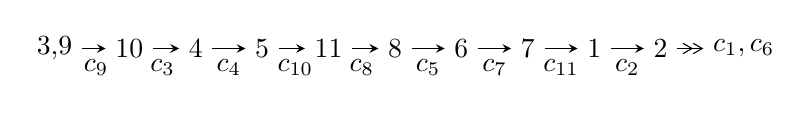
\begin{tikzpicture}[x=24pt, y=7pt]
	% node
	\node (A0) at (-1/8, 0) {3,9};
	\node (A1) at (1, 0) {10};
	\node (A2) at (2, 0) {4};
	\node (A3) at (3, 0) {5};
	\node (A4) at (4, 0) {11};
	\node (A5) at (5, 0) {8};
	\node (A6) at (6, 0) {6};
	\node (A7) at (7, 0) {7};
	\node (A8) at (8, 0) {1};
	\node (A9) at (9, 0) {2};
	\node (C1) at (1/2, -1) {$c_{9}$};
	\node (C2) at (3/2, -1) {$c_{3}$};
	\node (C3) at (5/2, -1) {$c_{4}$};
	\node (C4) at (7/2, -1) {$c_{10}$};
	\node (C5) at (9/2, -1) {$c_{8}$};
	\node (C6) at (11/2, -1) {$c_{5}$};
	\node (C7) at (13/2, -1) {$c_{7}$};
	\node (C8) at (15/2, -1) {$c_{11}$};
	\node (C9) at (17/2, -1) {$c_{2}$};
	\node (A10) at (41/4, 0) {$c_{1},c_{6}$};

	% edge
	\draw[->,>=stealth]	
	(A0) edge (A1) (A1) edge (A2) (A2) edge (A3) (A3) edge (A4) (A4) edge (A5) (A5) edge (A6) (A6) edge (A7) (A7) edge (A8) (A8) edge (A9) ;
	\draw[->>,>={angle 60}]	
	(A9) edge (A10);
\end{tikzpicture} \\ 

\end{tabular} \\

\footnotetext{
The image of knot diagram is generated by the software ``\textbf{Draw programme}" developed by Andrew Bartholomew(\url{http://www.layer8.co.uk/maths/draw/index.htm\#Running-draw}), where we modified some parts for our purpose(\url{https://github.com/CATsTAILs/LinksPainter}).
}\phantom \\ \newline 
\centering \textbf{Ideals for irreducible components\footnotemark of $X_{\text{par}}$} 
 
\begin{align*}
I^u_{1}&=\langle 
u^{44}- u^{43}+\cdots+2 u-1\rangle \\
\\
\end{align*}
\raggedright * 1 irreducible components of $\dim_{\mathbb{C}}=0$, with total 44 representations.\\
\footnotetext{All coefficients of polynomials are rational numbers. But the coefficients are sometimes approximated in decimal forms when there is not enough margin.}
\newpage
\renewcommand{\arraystretch}{1}
\centering \section*{I. $I^u_{1}= \langle u^{44}- u^{43}+\cdots+2 u-1 \rangle$}
\flushleft \textbf{(i) Arc colorings}\\
\begin{tabular}{m{7pt} m{180pt} m{7pt} m{180pt} }
\flushright $a_{3}=$&$\begin{pmatrix}0\\u\end{pmatrix}$ \\
\flushright $a_{9}=$&$\begin{pmatrix}1\\0\end{pmatrix}$ \\
\flushright $a_{10}=$&$\begin{pmatrix}1\\u^2\end{pmatrix}$ \\
\flushright $a_{4}=$&$\begin{pmatrix}- u\\- u^3+u\end{pmatrix}$ \\
\flushright $a_{5}=$&$\begin{pmatrix}u^3-2 u\\- u^3+u\end{pmatrix}$ \\
\flushright $a_{11}=$&$\begin{pmatrix}- u^2+1\\- u^4+2 u^2\end{pmatrix}$ \\
\flushright $a_{8}=$&$\begin{pmatrix}u^6-3 u^4+2 u^2+1\\- u^6+2 u^4- u^2\end{pmatrix}$ \\
\flushright $a_{6}=$&$\begin{pmatrix}u^9-4 u^7+5 u^5-3 u\\- u^9+3 u^7-3 u^5+u\end{pmatrix}$ \\
\flushright $a_{7}=$&$\begin{pmatrix}u^{12}-5 u^{10}+9 u^8-4 u^6-6 u^4+5 u^2+1\\u^{14}-6 u^{12}+13 u^{10}-10 u^8-4 u^6+8 u^4- u^2\end{pmatrix}$ \\
\flushright $a_{1}=$&$\begin{pmatrix}- u^{22}+9 u^{20}+\cdots+2 u^2+1\\- u^{24}+10 u^{22}+\cdots-4 u^4+2 u^2\end{pmatrix}$ \\
\flushright $a_{2}=$&$\begin{pmatrix}u^{42}-17 u^{40}+\cdots- u^2+1\\- u^{42}+16 u^{40}+\cdots+4 u^4+3 u^2\end{pmatrix}$\\ \flushright $a_{2}=$&$\begin{pmatrix}u^{42}-17 u^{40}+\cdots- u^2+1\\- u^{42}+16 u^{40}+\cdots+4 u^4+3 u^2\end{pmatrix}$\\&\end{tabular}
\flushleft \textbf{(ii) Obstruction class $= -1$}\\~\\
\flushleft \textbf{(iii) Cusp Shapes $= 4 u^{41}-64 u^{39}+\cdots+4 u-10$}\\~\\
\newpage\renewcommand{\arraystretch}{1}
\flushleft \textbf{(iv) u-Polynomials at the component}\newline \\
\begin{tabular}{m{50pt}|m{274pt}}
Crossings & \hspace{64pt}u-Polynomials at each crossing \\
\hline $$\begin{aligned}c_{1},c_{6}\end{aligned}$$&$\begin{aligned}
&u^{44}- u^{43}+\cdots+u^2-1
\end{aligned}$\\
\hline $$\begin{aligned}c_{2}\end{aligned}$$&$\begin{aligned}
&u^{44}+23 u^{43}+\cdots+2 u+1
\end{aligned}$\\
\hline $$\begin{aligned}c_{3},c_{9},c_{10}\end{aligned}$$&$\begin{aligned}
&u^{44}+u^{43}+\cdots-2 u-1
\end{aligned}$\\
\hline $$\begin{aligned}c_{4},c_{5},c_{8}\end{aligned}$$&$\begin{aligned}
&u^{44}-3 u^{43}+\cdots-10 u+5
\end{aligned}$\\
\hline $$\begin{aligned}c_{7},c_{11}\end{aligned}$$&$\begin{aligned}
&u^{44}-3 u^{43}+\cdots+70 u-7
\end{aligned}$\\
\hline
\end{tabular}\\~\\
\newpage\renewcommand{\arraystretch}{1}
\flushleft \textbf{(v) Riley Polynomials at the component}\newline \\
\begin{tabular}{m{50pt}|m{274pt}}
Crossings & \hspace{64pt}Riley Polynomials at each crossing \\
\hline $$\begin{aligned}c_{1},c_{6}\end{aligned}$$&$\begin{aligned}
&y^{44}-23 y^{43}+\cdots-2 y+1
\end{aligned}$\\
\hline $$\begin{aligned}c_{2}\end{aligned}$$&$\begin{aligned}
&y^{44}-3 y^{43}+\cdots-10 y+1
\end{aligned}$\\
\hline $$\begin{aligned}c_{3},c_{9},c_{10}\end{aligned}$$&$\begin{aligned}
&y^{44}-35 y^{43}+\cdots-2 y+1
\end{aligned}$\\
\hline $$\begin{aligned}c_{4},c_{5},c_{8}\end{aligned}$$&$\begin{aligned}
&y^{44}+41 y^{43}+\cdots-270 y+25
\end{aligned}$\\
\hline $$\begin{aligned}c_{7},c_{11}\end{aligned}$$&$\begin{aligned}
&y^{44}+29 y^{43}+\cdots-6454 y+49
\end{aligned}$\\
\hline
\end{tabular}\\~\\
\newpage\flushleft \textbf{(vi) Complex Volumes and Cusp Shapes}
$$\begin{array}{c|c|c}  
\text{Solutions to }I^u_{1}& \I (\text{vol} + \sqrt{-1}CS) & \text{Cusp shape}\\
 \hline 
\begin{aligned}
u &= \phantom{-}1.136420 + 0.070861 I\end{aligned}
 & -1.83859 - 0.36732 I & -5.44983 + 0.09330 I \\ \hline\begin{aligned}
u &= \phantom{-}1.136420 - 0.070861 I\end{aligned}
 & -1.83859 + 0.36732 I & -5.44983 - 0.09330 I \\ \hline\begin{aligned}
u &= \phantom{-}0.011664 + 0.857762 I\end{aligned}
 & \phantom{-}7.59511 - 2.36662 I & -0.82199 + 3.38645 I \\ \hline\begin{aligned}
u &= \phantom{-}0.011664 - 0.857762 I\end{aligned}
 & \phantom{-}7.59511 + 2.36662 I & -0.82199 - 3.38645 I \\ \hline\begin{aligned}
u &= -0.072887 + 0.852785 I\end{aligned}
 & \phantom{-}2.26398 + 8.63330 I & -5.49078 - 6.17544 I \\ \hline\begin{aligned}
u &= -0.072887 - 0.852785 I\end{aligned}
 & \phantom{-}2.26398 - 8.63330 I & -5.49078 + 6.17544 I \\ \hline\begin{aligned}
u &= \phantom{-}0.058073 + 0.845269 I\end{aligned}
 & \phantom{-}5.01784 - 3.75852 I & -2.18404 + 2.68935 I \\ \hline\begin{aligned}
u &= \phantom{-}0.058073 - 0.845269 I\end{aligned}
 & \phantom{-}5.01784 + 3.75852 I & -2.18404 - 2.68935 I \\ \hline\begin{aligned}
u &= -0.066510 + 0.814340 I\end{aligned}
 & \phantom{-}0.820194 + 0.338577 I & -7.27786 - 0.02628 I \\ \hline\begin{aligned}
u &= -0.066510 - 0.814340 I\end{aligned}
 & \phantom{-}0.820194 - 0.338577 I & -7.27786 + 0.02628 I \\ \hline\begin{aligned}
u &= -1.209090 + 0.176546 I\end{aligned}
 & -3.07255 + 4.10165 I & -9.63918 - 6.97252 I \\ \hline\begin{aligned}
u &= -1.209090 - 0.176546 I\end{aligned}
 & -3.07255 - 4.10165 I & -9.63918 + 6.97252 I \\ \hline\begin{aligned}
u &= -1.207320 + 0.344488 I\end{aligned}
 & -2.67222 + 3.85231 I & -10.89580 - 3.96243 I \\ \hline\begin{aligned}
u &= -1.207320 - 0.344488 I\end{aligned}
 & -2.67222 - 3.85231 I & -10.89580 + 3.96243 I \\ \hline\begin{aligned}
u &= -1.199240 + 0.400757 I\end{aligned}
 & -1.19898 - 4.13238 I & -8.61614 + 2.75656 I \\ \hline\begin{aligned}
u &= -1.199240 - 0.400757 I\end{aligned}
 & -1.19898 + 4.13238 I & -8.61614 - 2.75656 I \\ \hline\begin{aligned}
u &= \phantom{-}1.216460 + 0.389904 I\end{aligned}
 & \phantom{-}1.45135 - 0.67916 I & -5.37325 + 0. I\phantom{ +0.000000I} \\ \hline\begin{aligned}
u &= \phantom{-}1.216460 - 0.389904 I\end{aligned}
 & \phantom{-}1.45135 + 0.67916 I & -5.37325 + 0. I\phantom{ +0.000000I} \\ \hline\begin{aligned}
u &= -1.28385\phantom{ +0.000000I}\end{aligned}
 & -5.57163\phantom{ +0.000000I} & -16.6130\phantom{ +0.000000I} \\ \hline\begin{aligned}
u &= \phantom{-}1.261750 + 0.397871 I\end{aligned}
 & \phantom{-}3.71994 - 2.13541 I & \phantom{-0.000000 } 0 \\ \hline\begin{aligned}
u &= \phantom{-}1.261750 - 0.397871 I\end{aligned}
 & \phantom{-}3.71994 + 2.13541 I & \phantom{-0.000000 } 0 \\ \hline\begin{aligned}
u &= -1.280990 + 0.395746 I\end{aligned}
 & \phantom{-}3.57613 + 6.86218 I & \phantom{-0.000000 } 0 \\ \hline\begin{aligned}
u &= -1.280990 - 0.395746 I\end{aligned}
 & \phantom{-}3.57613 - 6.86218 I & \phantom{-0.000000 } 0 \\ \hline\begin{aligned}
u &= -1.336030 + 0.128402 I\end{aligned}
 & -5.89939 + 3.18300 I & -11.60255 + 0. I\phantom{ +0.000000I} \\ \hline\begin{aligned}
u &= -1.336030 - 0.128402 I\end{aligned}
 & -5.89939 - 3.18300 I & -11.60255 + 0. I\phantom{ +0.000000I} \\ \hline\begin{aligned}
u &= \phantom{-}1.353960 + 0.106974 I\end{aligned}
 & -9.55253 + 0.87557 I & -15.7624 + 0. I\phantom{ +0.000000I} \\ \hline\begin{aligned}
u &= \phantom{-}1.353960 - 0.106974 I\end{aligned}
 & -9.55253 - 0.87557 I & -15.7624 + 0. I\phantom{ +0.000000I} \\ \hline\begin{aligned}
u &= \phantom{-}1.354080 + 0.142889 I\end{aligned}
 & -9.09797 - 7.70313 I & -14.6073 + 0. I\phantom{ +0.000000I} \\ \hline\begin{aligned}
u &= \phantom{-}1.354080 - 0.142889 I\end{aligned}
 & -9.09797 + 7.70313 I & -14.6073 + 0. I\phantom{ +0.000000I} \\ \hline\begin{aligned}
u &= \phantom{-}1.314770 + 0.363443 I\end{aligned}
 & -3.50174 - 4.58387 I & \phantom{-0.000000 } 0\\
 \hline 
 \end{array}$$\newpage$$\begin{array}{c|c|c}  
\text{Solutions to }I^u_{1}& \I (\text{vol} + \sqrt{-1}CS) & \text{Cusp shape}\\
 \hline 
\begin{aligned}
u &= \phantom{-}1.314770 - 0.363443 I\end{aligned}
 & -3.50174 + 4.58387 I & \phantom{-0.000000 } 0 \\ \hline\begin{aligned}
u &= -1.312960 + 0.381210 I\end{aligned}
 & \phantom{-}0.73171 + 8.16553 I & \phantom{-0.000000 } 0 \\ \hline\begin{aligned}
u &= -1.312960 - 0.381210 I\end{aligned}
 & \phantom{-}0.73171 - 8.16553 I & \phantom{-0.000000 } 0 \\ \hline\begin{aligned}
u &= \phantom{-}1.322850 + 0.383944 I\end{aligned}
 & -2.10496 - 13.07590 I & \phantom{-0.000000 } 0 \\ \hline\begin{aligned}
u &= \phantom{-}1.322850 - 0.383944 I\end{aligned}
 & -2.10496 + 13.07590 I & \phantom{-0.000000 } 0 \\ \hline\begin{aligned}
u &= -0.371942 + 0.476818 I\end{aligned}
 & -3.72132 + 5.60891 I & -9.34455 - 7.77746 I \\ \hline\begin{aligned}
u &= -0.371942 - 0.476818 I\end{aligned}
 & -3.72132 - 5.60891 I & -9.34455 + 7.77746 I \\ \hline\begin{aligned}
u &= -0.442174 + 0.385790 I\end{aligned}
 & -4.03922 - 2.47426 I & -10.82917 - 0.27323 I \\ \hline\begin{aligned}
u &= -0.442174 - 0.385790 I\end{aligned}
 & -4.03922 + 2.47426 I & -10.82917 + 0.27323 I \\ \hline\begin{aligned}
u &= \phantom{-}0.334945 + 0.405418 I\end{aligned}
 & -0.74838 - 1.34331 I & -6.21576 + 4.98012 I \\ \hline\begin{aligned}
u &= \phantom{-}0.334945 - 0.405418 I\end{aligned}
 & -0.74838 + 1.34331 I & -6.21576 - 4.98012 I \\ \hline\begin{aligned}
u &= \phantom{-}0.101961 + 0.483460 I\end{aligned}
 & \phantom{-}0.81833 - 1.69616 I & -1.98579 + 6.04080 I \\ \hline\begin{aligned}
u &= \phantom{-}0.101961 - 0.483460 I\end{aligned}
 & \phantom{-}0.81833 + 1.69616 I & -1.98579 - 6.04080 I \\ \hline\begin{aligned}
u &= \phantom{-}0.348278\phantom{ +0.000000I}\end{aligned}
 & -0.869874\phantom{ +0.000000I} & -12.9060\phantom{ +0.000000I}\\
 \hline 
 \end{array}$$\newpage
\newpage\renewcommand{\arraystretch}{1}
\centering \section*{ II. u-Polynomials}
\begin{tabular}{m{50pt}|m{274pt}}
Crossings & \hspace{64pt}u-Polynomials at each crossing \\
\hline $$\begin{aligned}c_{1},c_{6}\end{aligned}$$&$\begin{aligned}
&u^{44}- u^{43}+\cdots+u^2-1
\end{aligned}$\\
\hline $$\begin{aligned}c_{2}\end{aligned}$$&$\begin{aligned}
&u^{44}+23 u^{43}+\cdots+2 u+1
\end{aligned}$\\
\hline $$\begin{aligned}c_{3},c_{9},c_{10}\end{aligned}$$&$\begin{aligned}
&u^{44}+u^{43}+\cdots-2 u-1
\end{aligned}$\\
\hline $$\begin{aligned}c_{4},c_{5},c_{8}\end{aligned}$$&$\begin{aligned}
&u^{44}-3 u^{43}+\cdots-10 u+5
\end{aligned}$\\
\hline $$\begin{aligned}c_{7},c_{11}\end{aligned}$$&$\begin{aligned}
&u^{44}-3 u^{43}+\cdots+70 u-7
\end{aligned}$\\
\hline
\end{tabular}\newpage\renewcommand{\arraystretch}{1}
\centering \section*{ III. Riley Polynomials}
\begin{tabular}{m{50pt}|m{274pt}}
Crossings & \hspace{64pt}Riley Polynomials at each crossing \\
\hline $$\begin{aligned}c_{1},c_{6}\end{aligned}$$&$\begin{aligned}
&y^{44}-23 y^{43}+\cdots-2 y+1
\end{aligned}$\\
\hline $$\begin{aligned}c_{2}\end{aligned}$$&$\begin{aligned}
&y^{44}-3 y^{43}+\cdots-10 y+1
\end{aligned}$\\
\hline $$\begin{aligned}c_{3},c_{9},c_{10}\end{aligned}$$&$\begin{aligned}
&y^{44}-35 y^{43}+\cdots-2 y+1
\end{aligned}$\\
\hline $$\begin{aligned}c_{4},c_{5},c_{8}\end{aligned}$$&$\begin{aligned}
&y^{44}+41 y^{43}+\cdots-270 y+25
\end{aligned}$\\
\hline $$\begin{aligned}c_{7},c_{11}\end{aligned}$$&$\begin{aligned}
&y^{44}+29 y^{43}+\cdots-6454 y+49
\end{aligned}$\\
\hline
\end{tabular}
\vskip 2pc
\end{document}